\chapter{Detailed Design and Implementation}
\pagestyle{fancy}

This chapter provides an exhaustive breakdown of the software engineering architecture, the hardware-accelerated algorithms, and the rigorous mathematical systems implemented to realize the \textit{ChronoLux} digital twin. Transitioning from theoretical radiometry and conservation physics into a highly performant desktop application requires a sophisticated orchestration of CPU scheduling, unmanaged memory transfers, and massive GPU parallelization. 

Predictive analysis workflows governed by the International Commission on Illumination (CIE) and Michalski guidelines for preventive conservation historically suffer from a lack of interactivity. Traditional offline software like Radiance demands hours of CPU-bound calculations for a single temporal simulation. \textit{ChronoLux} resolves this bottleneck by implementing a hybrid architecture utilizing the Unity 3D engine and the DirectX 12 graphics API to unlock hardware-accelerated DirectX Raytracing (DXR). This chapter systematically dissects each component of this pipeline, from mathematical astrometry to GPU memory management and asynchronous telemetry extraction.

\section{Software Architecture Overview}

To process the massive volume of ray queries required for an annual dosimetric simulation without halting the operating system, a strictly decoupled architecture is employed. The software stack is bifurcated into two distinct domains: the C\# CPU layer handling user interface, file I/O, deterministic structural sorting, and astrometric mathematics; and the HLSL Compute Shader layer executing the heavily parallelized Monte Carlo integrations directly on the GPU.

\begin{figure}[htbp]
	\centering
	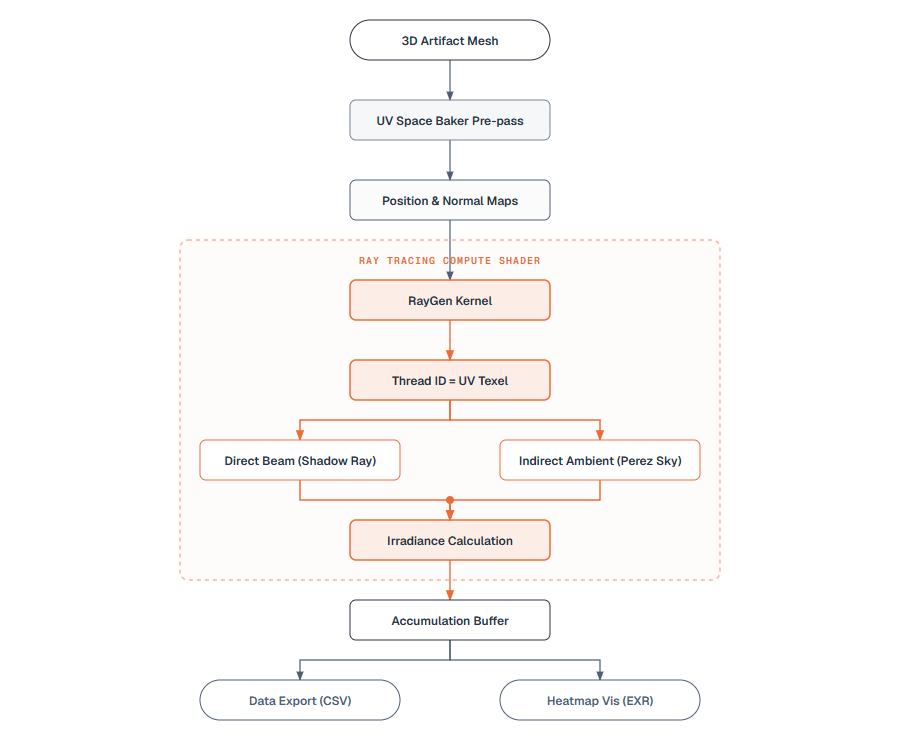
\includegraphics[width=\textwidth]{figures/pipeline.png}
	\caption{High-level simulation pipeline demonstrating the decoupling of CPU orchestration from GPU execution.}
	\label{fig:pipeline_diagram}
\end{figure}

\begin{figure}[htbp]
	\centering
	
\includegraphics[width=\textwidth]{figures/architecture.png}
	\caption{Overall Architectural System design of \textit{ChronoLux}, detailing data paths between the Engine, the GUI, and the OS filesystem.}
	\label{fig:architecture_diagram}
\end{figure}

As seen in Figures \ref{fig:pipeline_diagram} and \ref{fig:architecture_diagram}, the flow of data is strictly managed. Project parameters are serialized to JSON via the \texttt{ChronoProject} object, parsed by the \texttt{ProjectManager}, and fed into the \texttt{LightDoseSimulator}. This orchestrator acts as the simulation's beating heart, stepping time forward and delegating ray dispatching to the DXR kernels.

\section{Core Simulation Engine (C\# CPU Orchestration)}

The core logic of the application must ensure mathematical determinism, prevent hardware starvation, and respond dynamically to user inputs.

\begin{figure}[htbp]
	\centering
	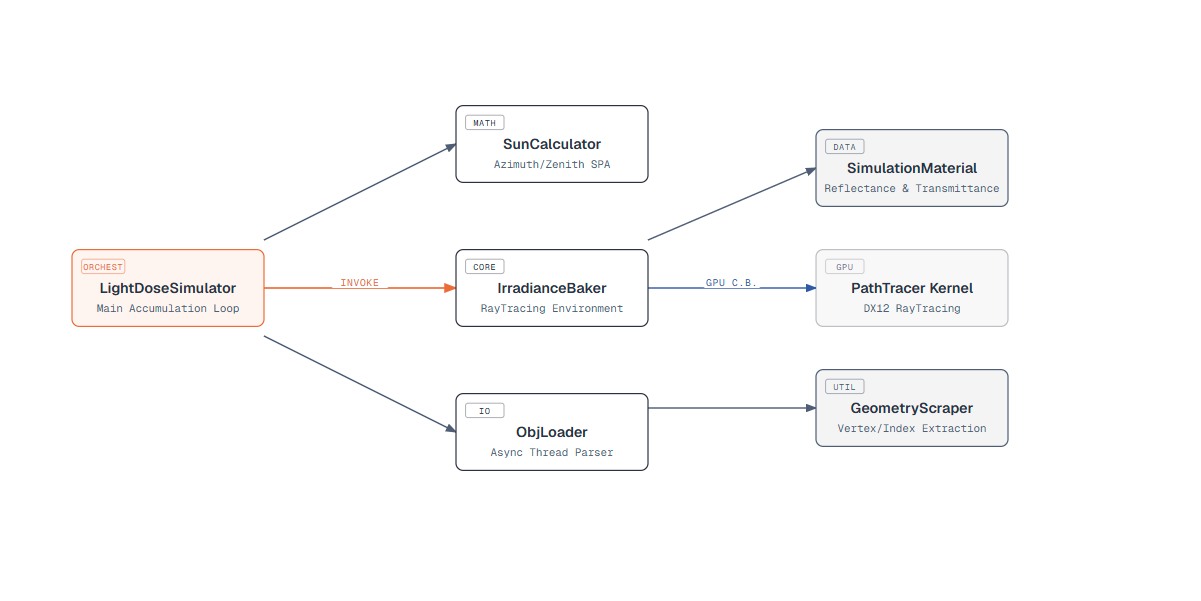
\includegraphics[width=\textwidth]{figures/csharp_class_diagram.png}
	\caption{C\# CPU Class Architecture and Data Flow orchestration within \textit{ChronoLux}.}
	\label{fig:csharp_class_diagram}
\end{figure}

As shown in Figure \ref{fig:csharp_class_diagram}, the \texttt{LightDoseSimulator} depends on several critical sub-systems: \texttt{SunCalculator} for astrometric mathematics, \texttt{IrradianceBaker} for hardware dispatching, and \texttt{RuntimeModelLoader} for asynchronous file I/O.

\subsection{The Chronological Engine and Time Stepping}

The primary responsibility of the \texttt{LightDoseSimulator} is to advance the master clock $\Delta t$ and generate the precise solar altitude and azimuth required for the Perez sky model. 

The simulation logic must process an entire meteorological year while preventing the Operating System from triggering a Timeout Detection and Recovery (TDR) crash, which forcefully restarts the graphics driver if a single task takes longer than approximately 2 seconds. This is achieved via a C\# \texttt{IEnumerator} Coroutine (\texttt{RunSimulationInternal}). As detailed in Appendix \ref{apx:csharp_code} (Listing \ref{lst:timeloop}), the time-stepping loop is entirely dynamic. It processes the user-defined \texttt{startDay} and \texttt{endDay} linearly. 

For every single day, the Coroutine utilizes the \texttt{SunCalculator} to dynamically query the exact local sunrise and sunset boundaries based on the user's defined latitude, longitude, and UTC offset. This prevents the simulation from wasting cycles tracing rays in the middle of the night. If the calculated sunrise and sunset times are identical (an edge case during polar nights at extreme latitudes), the simulation intelligently skips the entire day.

An aggressive computational culling strategy is further employed inside the hourly step loop. The engine skips any temporal step where both the incoming direct beam lux and the diffuse sky lux are calculated to be functionally zero (specifically $< 0.1$ Lux). By omitting these low-energy twilight steps where atmospheric scattering absorbs nearly all solar irradiance, \textit{ChronoLux} saves millions of unnecessary Monte Carlo ray casts per simulated year, directly boosting overall performance. 

During active simulation periods, the Coroutine explicitly uses the \texttt{yield return null;} statement. This instruction pauses the Coroutine's execution until the next engine frame, actively yielding the thread back to the Unity main loop. This guarantees that the UI remains fully responsive, the progress bar animates smoothly, and the TDR watchdog is appeased.

\subsection{Mathematical Astrometry and Solar Ephemeris}

Achieving metrological accuracy requires precise solar positioning at every hour of the year. The \texttt{SunCalculator.cs} class implements rigorous celestial mathematical models, determining not only the vector position of the solar disc but also evaluating atmospheric attenuation to yield physically accurate \texttt{BeamLux} and \texttt{DiffuseLux} values.

The first step converts the local simulation time into a Julian Day (JD) epoch, calculating Julian centuries $T$ from J2000.0. The geometric mean longitude ($L_0$) and mean anomaly ($M$) of the sun are given by:
\begin{equation}
L_0 = \left(280.46646 + T(36000.76983 + T \times 0.0003032)\right) \pmod{360^\circ}
\end{equation}
\begin{equation}
M = 357.52911 + T(35999.05029 - 0.0001537 \times T)
\end{equation}

To account for Earth's orbital eccentricity, the Equation of Center ($C$) is derived using Fourier series expansion, which corrects the geometric mean longitude to the apparent longitude ($\lambda_{app}$):
\begin{equation}
C = \sin(M)(1.914602 - 0.004817 T) + \sin(2M)(0.019993) + \sin(3M)(0.000289)
\end{equation}

The Mean Obliquity of the Ecliptic ($\epsilon_0$) is corrected for nutation to calculate the Solar Declination ($\delta$), defining how far the sun resides above or below the celestial equator:
\begin{equation}
\delta = \arcsin\left(\sin(\epsilon) \sin(\lambda_{app})\right)
\end{equation}

With $\delta$ established, the Equation of Time ($EqT$) maps solar time to clock time. Combining $EqT$ with the terrestrial longitude yields the True Solar Time (TST) and the Hour Angle ($H$):
\begin{equation}
H = \frac{TST}{4.0} - 180^\circ
\end{equation}

Finally, the Solar Zenith Angle ($\theta_z$) and Azimuth ($\phi$) are strictly defined relative to the user's latitude ($\Phi$):
\begin{equation}
\cos(\theta_z) = \sin(\Phi)\sin(\delta) + \cos(\Phi)\cos(\delta)\cos(H)
\end{equation}

With the astrometric vector position fixed, the clear-sky direct beam irradiance ($E_{beam}$) is computed using the rigorous Kasten-Young formula for optical air mass ($AM$). As the sun approaches the horizon, the thickness of the atmosphere the light must penetrate increases non-linearly:
\begin{equation}
AM = \frac{1}{\sin(\alpha) + 0.50572(\alpha + 6.07995)^{-1.6364}}
\end{equation}
\begin{equation}
E_{beam} = 127500 \times 0.7^{AM^{0.678}} \quad [\text{Lux}]
\end{equation}
Where $\alpha$ is the solar altitude angle ($90^\circ - \theta_z$), and $0.7$ acts as the baseline atmospheric transmittance coefficient for clear-sky conditions.
For ambient lighting, a simplified Haurwitz clear-sky diffuse model calculates horizontal diffuse illuminance ($E_{diffuse}$), estimating atmospheric scattering based on the total potential solar constant versus direct atmospheric penetration. These precise \texttt{BeamLux} and \texttt{DiffuseLux} values are injected directly into the HLSL compute kernel for every single time step.

\section{Scene Management and Hardware Interfaces}

\subsection{Asynchronous Runtime Mesh Parsing}

Because \textit{ChronoLux} is distributed as a compiled desktop metrology application, it cannot rely on pre-compiled Unity Scene assets. It must dynamically load arbitrary, user-provided \texttt{.obj} files at runtime from the local filesystem. Heritage artifacts, such as laser-scanned church interiors or high-resolution photogrammetry models, can easily exceed several million vertices. If a string-based parser attempted to read these files synchronously on the main Unity thread, the application would permanently freeze, and the OS would terminate it with an "Application Not Responding" failure.

As demonstrated in Appendix \ref{apx:csharp_code} (Listing \ref{lst:objloader}), the \texttt{RuntimeModelLoader.cs} resolves this memory bottleneck by implementing a heavily threaded chunk parser. The reading of the file and the string parsing of vertices, normals, and UV coordinates occurs entirely inside a \texttt{Task.Run()} background thread executing on separate logical CPU cores. 
While this parse task runs in the background, the main thread loop evaluates a \texttt{while (!parseTask.IsCompleted)} condition, repeatedly calling \texttt{yield return null;} and updating the \texttt{ProgressBar} UI element via \texttt{UpdateProgress()}. Only once the massive memory arrays are fully populated is execution yielded back to the Unity main thread for the final \texttt{Mesh.SetVertices()} upload to VRAM and the subsequent \texttt{GameObject} generation. This architecture keeps the UI fully responsive during the heaviest data loads.

\subsection{Dynamic Material Serialization and Hierarchy Keying}

When a heritage artifact is loaded via the runtime loader, the original materials are completely stripped. Instead, the simulation maps physically validated presets (e.g., Brick, Hardwood, Antique Glass) onto the individual sub-meshes. This mapping is securely persisted in the \texttt{ChronoProject} JSON file.

To re-apply these materials safely across different application sessions, the \texttt{RuntimeModelLoader} uses a unique string keying mechanism. Relying purely on a \texttt{GameObject}'s name is insufficient because `.obj` files often contain duplicate component names like \texttt{Wall} or \texttt{Window\_01}. The \texttt{GetObjectKey} function constructs a distinct hierarchical identifier:
\begin{lstlisting}[language={[Sharp]C}]
private string GetObjectKey(GameObject go) {
    if (go.transform.parent != null && go.transform.parent != modelRoot)
        return $"{go.transform.parent.name}/{go.name}";
    return go.name;
}
\end{lstlisting}
This \texttt{RootName/MeshName} composite key guarantees that when the \texttt{ApplySavedMaterial} logic iterates over the loaded mesh components, it securely matches the geometry against the serialized \texttt{project.objectNames} array and retrieves the exact GUID for the \texttt{project.materialPresetNames}, completely avoiding material crossover errors.

\subsection{Spatial Normalization}

Imported geometries exhibit extreme variations in scale; some architectural models are constructed in millimeters, others in meters, and some geographic surveys in kilometers. To prevent catastrophic floating-point precision loss inside the DXR kernel—which occurs when rays must intersect extremely large coordinate spaces—\textit{ChronoLux} applies a strict spatial normalization pipeline via the \texttt{CenterAndScaleModel} function.

The algorithm calculates the global bounding box encapsulating all sub-meshes attached to the artifact root. It determines the maximum dimensional span:
\begin{equation}
MaxDim = \max(Width, \max(Height, Depth))
\end{equation}
A uniform scaling factor is then calculated: $Factor = 2.0 / MaxDim$ (assuming $MaxDim > 0$). Every child vertex transform is then translated so the object's mathematical centroid rests exactly at local $(0,0,0)$, and scaled uniformly by the $Factor$. This mathematical normalization guarantees that the entire heritage site, regardless of its original CAD scale, strictly occupies a 2.0-meter bounding box in World Space. 
Because the DXR ray tracer relies on 32-bit floating point math, keeping intersection geometry strictly within the $[-1.0, 1.0]$ bounds near the origin maximizes the IEEE 754 mantissa precision, preventing "shadow acne" and geometric clipping. The user's semantic transformations (position and scale offsets loaded from the \texttt{ChronoProject} JSON) are then applied exclusively to the normalized root object.

\subsection{Deterministic BVH Building}

As highlighted in theoretical radiometry literature, Monte Carlo integration is susceptible to floating-point associativity errors. However, an even greater threat in a hybrid CPU-GPU engine is structural non-determinism. Unity's \texttt{FindObjectsByType<Renderer>()} API does not guarantee a strictly deterministic return order across different operating systems or CPU architectures. If the mapping between a ray's geometric \texttt{InstanceID} and its underlying physical \texttt{SimulationMaterial} shifts between runs, the dosimetric simulation loses all scientific reproducibility.

To resolve this, the \texttt{IrradianceBaker.cs} initialization enforces strict determinism by collecting all active \texttt{Renderer} components and explicitly sorting them using a deeply granular $O(n \log n)$ string-based ordinal comparison. The unique \texttt{SortKey} for every sub-mesh is constructed as follows:
\begin{equation}
\text{SortKey} = \text{ScenePath} \,|\, \text{TransformHierarchy} \,|\, \text{Type} \,|\, \text{MaterialSlot}
\end{equation}
The \texttt{TransformHierarchy} is built by recursively ascending the parent tree and appending the exact \texttt{GetSiblingIndex()} padded to 6 digits (e.g., \texttt{000002:Wall/000000:Window}). This incredibly stable ordinal sort guarantees that the structural Index and Vertex buffers uploaded to the GPU, alongside the \texttt{\_SimulationMaterials} \texttt{StructuredBuffer}, are mathematically identical and perfectly aligned across entirely different hardware platforms, ensuring absolute reproducibility in lux-hour accumulation.

\section{Hardware-Accelerated Path Tracing (HLSL / DXR)}

The true computational bottleneck of \textit{ChronoLux} lies within the ray tracing logic. For every pixel in the artifact's UV map, stochastic rays must be cast to evaluate the rendering equation over thousands of simulated hours.

\subsection{Memory Management and DXR Acceleration Structures}

DirectX Raytracing relies on a hardware-accelerated two-tier hierarchy: the Bottom-Level Acceleration Structure (BLAS) storing raw triangle data, and the Top-Level Acceleration Structure (TLAS) defining spatial instances of the BLAS. In \textit{ChronoLux}, the TLAS is built and managed via Unity's \texttt{RayTracingAccelerationStructure}. 

Memory is strictly managed to align with GPU 16-byte boundaries. Data blocks transferred to the graphics card must obey HLSL packing rules to prevent memory corruption. For example, the \texttt{MeshMetadata} struct is explicitly padded inside C\# to ensure an exact 16-byte footprint:
\begin{lstlisting}[language={[Sharp]C}]
[StructLayout(LayoutKind.Sequential)]
private struct MeshMetadata {
    public uint vertexOffset;  // 4 bytes
    public uint indexOffset;   // 4 bytes
    public uint hasGeometry;   // 4 bytes
    public uint padding;       // 4 bytes (Forcing 16-byte alignment)
}
\end{lstlisting}
Similarly, the GPU expects \texttt{float4} structures for optimal SIMD (Single Instruction, Multiple Data) processing lanes. As a result, the \texttt{\_NormalMap} texture utilizes all four channels, storing the geometric $(x,y,z)$ coordinates in the RGB channels, while reserving the alpha channel ($w$) as a strictly binary coverage flag indicating valid geometry versus empty padding space.

The \texttt{SimulationMaterial} variables (reflectance, transmittance) are packed into \texttt{Vector4} arrays and mapped into the \texttt{\_SimulationMaterials} \texttt{ComputeBuffer}. When the \texttt{IrradianceBaker} builds the TLAS using \texttt{rtas.AddInstance()}, it applies specific flags. Sub-meshes are assigned \texttt{RayTracingSubMeshFlags.ClosestHitOnly}. This hardware optimization disables the invocation of "Any-Hit" shaders during traversal, significantly improving silicon performance since the simulation only requires the absolute nearest geometric intersection point.

\begin{figure}[htbp]
	\centering
	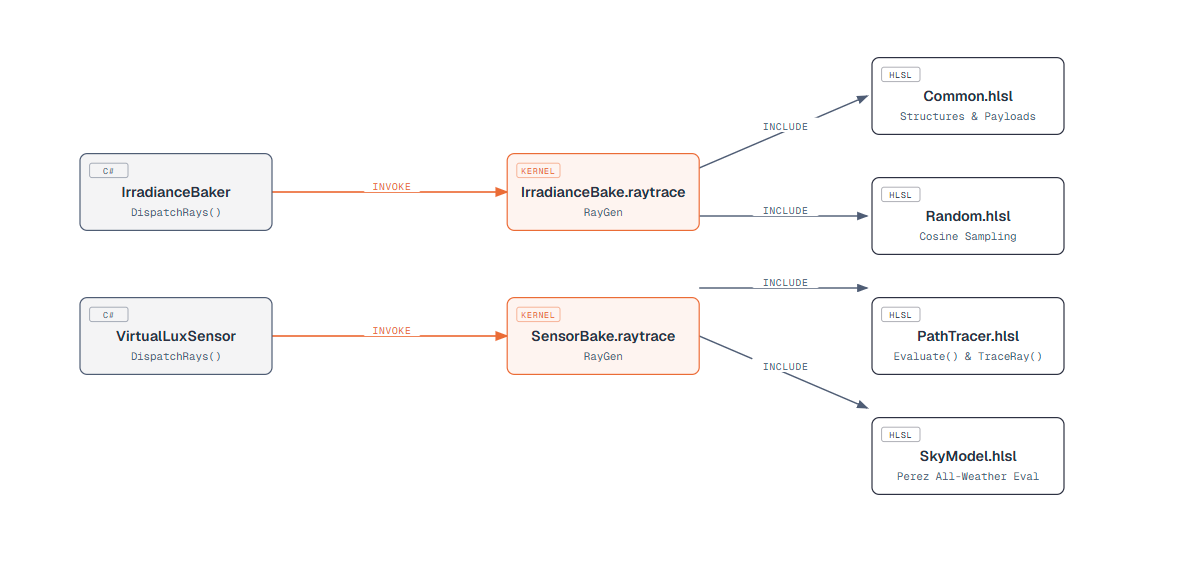
\includegraphics[width=\textwidth]{figures/shader_class_diagram.png}
	\caption{HLSL Compute Shader modular structure and inclusion tree.}
	\label{fig:shader_class_diagram}
\end{figure}

\subsection{Texture Space Dispatch Paradigm}

\textit{ChronoLux} drastically diverges from traditional screen-space video game graphics by utilizing Texture Space Ray Tracing. Instead of firing primary rays from the user's virtual camera lens towards a 1080p screen grid (which would only accumulate dose for pixels currently visible to the user), the compute kernel maps threads directly to the two-dimensional $(u,v)$ coordinates of the target mesh's unrolled UV layout.

\begin{figure}[H]
    \begin{algorithmic}
        \Require $PosMap, NormMap, SunDir, N_{samples}, \Delta t$
        \For{\textbf{each} thread $id \in \text{DispatchThreadID}$}
        \State $\mathbf{p} \leftarrow PosMap[id].xyz$
        \State $\mathbf{n} \leftarrow NormMap[id].xyz$
        \If{$\text{length}(\mathbf{n}) < 0.1$}
        \State \textbf{return} \quad \text{// Terminate thread (empty UV padding)}
        \EndIf
        
        \State $E_{dir} \leftarrow 0$
        \State $NdotL \leftarrow \mathbf{n} \cdot SunDir$
        \If{$NdotL > 0.0$}
        \State $E_{dir} \leftarrow \textsc{TracePath}(\mathbf{p}, SunDir, \dots, \text{isDirectSun=true}) \times NdotL$
        \EndIf
        
        \State $E_{ind} \leftarrow 0$
        \For{$i = 1$ \textbf{to} $N_{samples}$}
        \State $\omega_i \leftarrow \textsc{GetCosineWeightedDirection}(\mathbf{n})$
        \State $E_{ind} \leftarrow E_{ind} + \textsc{TracePath}(\mathbf{p}, \omega_i, \dots, \text{isDirectSun=false})$
        \EndFor
        
        \State $E_{total} \leftarrow E_{dir} + (E_{ind} / N_{samples}) \cdot \pi$
        
        \State $DoseMap[id] \leftarrow DoseMap[id] + E_{total} \cdot \Delta t$
        \State $DirectDoseMap[id] \leftarrow DirectDoseMap[id] + E_{dir} \cdot \Delta t$
        \State $IndirectDoseMap[id] \leftarrow IndirectDoseMap[id] + (E_{ind} / N_{samples}) \cdot \pi \cdot \Delta t$
        \EndFor
    \end{algorithmic}
    \caption{Pseudocode for Texture Space Ray Tracing dispatch separated into Direct and Stochastic Multi-Sampling paths.}
    \label{alg:ts_raytrace}
\end{figure}

A pre-pass baker uses the standard rasterization pipeline to write the world-space positions ($P$) and geometric normals ($N$) into \texttt{\_PositionMap} and \texttt{\_NormalMap} textures. As shown in Algorithm \ref{alg:ts_raytrace} (and detailed in Appendix \ref{apx:pathtracer_code}), the ray generation kernel (\texttt{IrradianceBakeRayGen}) is dispatched across this 2D grid. If a pixel has a normal length near zero, it indicates empty void space in the UV padding, and the thread terminates instantly to save cycles. Otherwise, the kernel uses $P$ and $N$ as the origin and orientation for the evaluation of the rendering equation. This architecture makes light simulation completely detached from screen space, permanently baking energy data directly onto the architectural surface.

\subsection{Pseudo-Random Sequence Generation and Hashing}

Monte Carlo integration fundamentally relies on uniform random sampling across the target domain (the celestial hemisphere). If the random number generator exhibits clustering or spatial-temporal correlations, the rendering equation evaluation becomes biased, manifesting as structural noise patterns rather than a uniform reduction in variance.

To resolve this inside the HLSL kernel without the overhead of tracking massive state arrays, \textit{ChronoLux} implements a stateless hashing algorithm bound to the thread's pixel coordinate ($x, y$) and the active simulation time step ($\Delta t$). 
\begin{equation}
\text{baseSeed} = \text{Hash}(id.y \times \text{dims}.x + id.x + \text{\_FrameIndex})
\end{equation}
By directly injecting \texttt{\_FrameIndex} (a sequentially increasing integer tracking the specific temporal step) into the core integer hash, the generated sequence of stochastic multi-samples shifts continuously throughout the year. As hundreds of time steps accumulate into the single \texttt{\_DoseMap} buffer, the high-frequency noise mathematically cancels itself out, allowing the Monte Carlo estimator to organically converge towards the true ground-truth irradiance integral.

\subsection{Direct Sunlight and Stochastic Multi-Sampling Paths}

To accurately evaluate the ambient light bouncing through the environment, \textit{ChronoLux} distinctly splits the integration into two explicit paths inside the ray generation shader.

The first path handles \textbf{Direct Sun}. If the surface normal faces the solar vector (\texttt{nDotSun > 0.0}), a single specific ray is fired directly towards the analytical sun vector by calling \texttt{TracePath} with \texttt{isDirectSun = true}. Inside \texttt{PathTracer.hlsl}, direct rays are uniquely allowed to traverse through transparent geometry. If the direct ray hits a material, the hardware queries the \texttt{\_SimulationMaterials} buffer for \texttt{transmittance}. If transmittance is greater than zero (e.g., stained glass), the throughput multiplier is attenuated by the transmittance value, the ray origin is nudged explicitly forward, and the ray continues its traversal through the object towards the sun. If transmittance is zero, it acts as an opaque shadow caster, and the traversal immediately returns $0.0$ lux.

The second path handles \textbf{Indirect Ambient Bouncing} via Stochastic Multi-Sampling. For every pixel, a \texttt{for}-loop generates $N_{samples}$ pseudo-random vectors over the hemisphere utilizing Cosine-Weighted Importance Sampling (\texttt{GetCosineWeightedDirection}). These rays call \texttt{TracePath} with \texttt{isDirectSun = false}. 

Unlike direct rays, indirect rays utilize the probabilistic \textbf{Russian Roulette} path termination technique. Russian Roulette provides an unbiased mathematical framework for terminating infinite recursive bounces without arbitrarily clipping light energy. At each bounce intersection, a random float $rv \in [0, 1)$ is generated from the hash sequence. Based on the material's scalar \texttt{reflectance} ($R$) and \texttt{transmittance} ($T$), the ray's fate is decided via cumulative probability thresholds:
\begin{enumerate}
    \item \textbf{Reflection ($rv < R$)}: The ray survives and generates a new cosine-weighted hemisphere vector.
    \item \textbf{Transmission ($rv < R + T$)}: The ray passes directly through the surface geometry without deviating its trajectory.
    \item \textbf{Absorption ($rv \geq R + T$)}: The ray is probabilistically absorbed by the material, and the path is immediately terminated.
\end{enumerate}

Because the ray only continues its trajectory when it mathematically "survives" the material's properties, the throughput does not need to be manually divided by the reflection multiplier at every vertex—the probability of survival itself acts as the exact energy attenuation weighting factor. If an indirect ray escapes the bounding volume hierarchy (BVH) without being fully absorbed, it triggers the \texttt{EvaluateSky()} function, tapping into the Perez Sky Model to fetch physically accurate atmospheric luminance. This deeply recursive behavior allows \textit{ChronoLux} to accurately calculate highly occluded indirect lighting scenarios, such as light bouncing down a hallway or reflecting off a highly reflective marble floor onto a textile artifact.

\section{Advanced Mathematical Models and Optimization}

To ensure the scientific validity and computational feasibility of the simulation, several advanced mathematical paradigms and hardware optimizations are integrated into the \textit{ChronoLux} engine.

\subsection{Perez Sky Model Atmospheric Coefficients}

While the direct solar disc dictates the intense beam irradiance, the vast majority of complex architectural ambient lighting is driven by diffuse sky scattering. \textit{ChronoLux} evaluates this using the Perez All-Weather Sky Model (\texttt{SkyModel.hlsl}), which models the highly anisotropic luminance of the celestial dome.

The engine implements the model for a clear sky with a Turbidity of $T=2.0$, utilizing five empirically derived static coefficients:
\begin{itemize}
    \item $a = -0.1058$: Dictates horizon brightening or darkening.
    \item $b = -0.0738$: Controls the luminance gradient near the horizon.
    \item $c = 1.8200$: Defines the relative intensity of the circumsolar corona.
    \item $d = -2.9744$: Controls the spatial width of the circumsolar region.
    \item $e = 0.1778$: Defines the backward scattered light opposing the sun.
\end{itemize}

Whenever an indirect stochastic ray misses all geometry, the zenith angle ($\theta$) and the angular distance to the sun ($\gamma$) are calculated. The relative luminance is evaluated via the scattering indicatrix function:
\begin{equation}
f(\theta, \gamma) = \left[1 + a \exp\left(\frac{b}{\cos\theta}\right)\right] \times \left[1 + c \exp(d \gamma) + e \cos^2\gamma\right]
\end{equation}
The result is then normalized against the dynamically calculated \texttt{DiffuseLux} provided by the CPU astrometry system (via the normalization factor $E_{diffuse} \times 0.2$). This evaluates to a physically accurate spectral distribution that perfectly mimics real-world atmospheric scattering.

\subsection{Hardware Traversal Mechanics (DXR and Face Culling)}

The decision to build \textit{ChronoLux} strictly upon DirectX 12 DXR fundamentally shifts the traversal bottleneck from software to raw silicon. Modern desktop GPUs feature dedicated Ray Tracing Cores that natively accelerate the traversal of the BVH tree and the complex Moeller-Trumbore ray-triangle intersection mathematical tests.

Furthermore, when the \texttt{TraceRay} HLSL intrinsic is called for direct sunlight shadows, a specific ray flag is injected into the payload structure: \texttt{RAY\_FLAG\_CULL\_BACK\_FACING\_TRIANGLES}. Because direct shadow rays only care about binary occlusion (is the sun visible or blocked?), and since architectural CAD models are typically closed manifolds (e.g., a wall has two sides), this hardware flag immediately discards intersection tests against any triangle facing away from the ray origin. This halves the computational burden on the RT Cores for shadow evaluation. Crucially, this optimization is explicitly disabled for indirect multi-bounce rays, as light must be able to reflect off the interior back-faces of transparent geometry like display cases.

\section{Asynchronous Data Telemetry and UI Integration}

\subsection{Automated Sensor Placement}

In physical metrology, scientists place physical lux meters around the laboratory. In the digital twin, \textit{ChronoLux} mimics this behavior by deploying \texttt{VirtualLuxSensor} objects. 
To guarantee objective baseline measurements, the \texttt{RuntimeModelLoader} automates the placement of an outdoor reference sensor array. When an environment model is loaded, the engine invokes \texttt{CreateOutdoorReferenceSensors}. This function iterates across all renderers to calculate a global master bounding box enclosing the entire heritage site. It derives the highest spatial point ($Y_{max} + 2.0\text{m}$) and the total geometric radius. Five sensors are then spawned automatically—one directly in the center, and four arranged in a complete perimeter circle. This ensures that regardless of the complexity of the CAD artifact below, there will always be unobscured sensors tracking the unadulterated baseline sunlight potential for that specific latitude and day.

\subsection{Metrological Analytics Pipeline}

True scientific metrology requires raw, extractable numerics. The quantitative availability of precise light dose metrics is critical for subsequent statistical analysis in Excel or Python. The application relies on an asynchronous, headless telemetry extraction pipeline to move high-resolution floating-point data from VRAM back to the CPU without stuttering the 60 FPS render cycle.

\begin{figure}[H]
    \begin{algorithmic}
        \Require $\text{DownsampleRT}, \text{DirectRT}, \text{IndirectRT}$
        \State $\text{completedRequests} \leftarrow 0$
        \State $\text{Trigger AsyncGPUReadback.Request}(\text{DownsampleRT})$
        \State $\text{Trigger AsyncGPUReadback.Request}(\text{DirectRT})$
        \State $\text{Trigger AsyncGPUReadback.Request}(\text{IndirectRT})$
        
        \While{$\text{completedRequests} < 3$}
            \State \textbf{Wait asynchronously} (Non-blocking)
        \EndWhile
        
        \State $\text{data} \leftarrow \text{Extract } float \text{ arrays}$
        \State $MaxDose \leftarrow 0, \mu \leftarrow 0, \text{CoverageCount} \leftarrow 0, N_{active} \leftarrow 0$
        
        \For{$i = 0$ \textbf{to} $65536$} \quad \text{// Iterating 256x256 buffer}
            \State $val \leftarrow \text{data}[i]$
            \If{$val > 0.0$}
                \State $N_{active} \leftarrow N_{active} + 1$
                \State $\mu \leftarrow \mu + val$
                \If{$val > MaxDose$} $MaxDose \leftarrow val$ \EndIf
                \If{$val > \text{Threshold}$} $\text{CoverageCount} \leftarrow \text{CoverageCount} + 1$ \EndIf
            \EndIf
        \EndFor
        
        \State $\mu \leftarrow \mu / N_{active}$
        \State $\text{CoveragePercent} \leftarrow (\text{CoverageCount} / N_{active}) \times 100$
    \end{algorithmic}
    \caption{CPU-Side Asynchronous Readback loop computing total scene variance and coverage metrics without blocking the primary rendering thread.}
    \label{alg:async_readback}
\end{figure}

Iterating sequentially over a $1024\times1024$ float array every single simulated hour on the CPU would devastate performance. To resolve this, \texttt{LightDoseSimulator.cs} utilizes hardware \texttt{Graphics.Blit} downsampling. Three heavily downscaled $256\times256$ RenderTextures (\texttt{\_downsampleRT}, \texttt{\_directDownsampleRT}, \texttt{\_indirectDownsampleRT}) are generated natively on the GPU.

Instead of blocking the thread, the C\# system invokes Unity's \texttt{AsyncGPUReadback.Request}. As demonstrated in Algorithm \ref{alg:async_readback}, this schedules a direct memory access (DMA) transfer. A callback closure tracks a \texttt{completed} counter. Only when the counter reaches 3 (signifying all three buffers have successfully arrived in system RAM) does the CPU retrieve the underlying float arrays: \texttt{req.GetData<float>().ToArray()}. 

Once the float arrays are safely on the CPU, a highly optimized memory loop iterates over the $65,536$ downscaled pixels. It computes the absolute maximum dose exposure, counts the number of strictly active pixels to derive the arithmetic mean ($\mu$), and tracks exactly how many pixels have crossed the user-defined \texttt{coverageThreshold} (e.g., 50,000 Lux-Hours for delicate watercolor paintings). By maintaining distinct arrays for Direct and Indirect accumulation, the telemetry framework allows conservators to isolate exact sources of UV/Visible energy damage.

\subsection{User Interface Toolkit and JSON Serialization Constraints}

The graphical interface of \textit{ChronoLux} is built utilizing Unity's modern UI Toolkit (UXML/USS), replacing the legacy Canvas immediate-mode GUI with a strict Model-View-Controller (MVC) DOM-based architecture. This responsive framework ensures the interface scales flawlessly across 4K laboratory monitors.

Scientific reproducibility dictates that experimental parameters must be precisely savable. The \texttt{ProjectManager.cs} system employs a custom JSON serialization engine via \texttt{JsonUtility}. However, architecting this serialization pipeline presented a significant software engineering challenge: Unity's native \texttt{JsonUtility} explicitly does not support the serialization of standard C\# \texttt{Dictionary<TKey, TValue>} collections. 

To bypass this engine limitation without resorting to heavy third-party JSON libraries (which would bloat the executable), the \texttt{ChronoProject} architecture implements a structural data flattening technique. Instead of saving a dictionary mapping a sub-mesh's string key directly to its material GUID, the data is manually split into two perfectly synchronized, parallel lists:
\begin{lstlisting}[language={[Sharp]C}]
[Serializable]
public class ChronoProject {
    public string projectName;
    public string artifactPath;
    
    // Parallel arrays resolving Dictionary serialization limits
    public List<string> objectNames = new List<string>();
    public List<string> materialPresetNames = new List<string>();
}
\end{lstlisting}

When an experiment is saved, the \texttt{ProjectManager} iterates over the active simulation hierarchy, extracting the \texttt{RootName/MeshName} keys and pushing them into the \texttt{objectNames} array, while simultaneously pushing the corresponding Material GUID into the \texttt{materialPresetNames} array at the exact same index. When the project is later loaded, a reconstruction loop dynamically rebuilds the C\# dictionary in local memory before applying it to the DXR \texttt{IrradianceBaker}. Due to the complexity of the data—including nested string-based hierarchy paths mapped to specific Material GUIDs and spatial roots—the JSON format provides a human-readable experimental manifest. 

When an experiment is launched, the data flows in a strictly unidirectional pattern: the \texttt{LightDoseSimulator} calculates astrometric variables, updates its internal C\# Model, and triggers UI property-changed events. The UI Controller intercepts these updates to refresh the DOM view. This architectural separation ensures that the intensive background math calculations never directly mutate the UI layout, maintaining a strict Model-View boundary.

\section{Deep Engine Optimizations and Memory Integrity}

Scaling a dosimetric ray tracer to process millions of rays per frame demands extreme optimization. Several low-level engine mechanics must be carefully orchestrated to maintain fidelity and hardware stability over an 8,760-hour simulation.

\subsection{Ray-Origin Epsilon Offsetting and Floating Point Limits}

A fundamental mathematical vulnerability of ray tracing architectures involves IEEE 754 floating-point truncation. When an intersection is identified by the BVH, the new ray origin is placed precisely on the mathematical surface of the triangle. Due to limited 32-bit float precision, the calculated point might mathematically fall slightly \textit{inside} the geometry. If the next bounce ray is cast from this point, it will immediately intersect the triangle it originated from, causing massive "shadow acne" artifacts that destroy dosimetric validity.

To prevent this, \textit{ChronoLux} implements a strict normal-based epsilon offset inside \texttt{PathTracer.hlsl}. 
\begin{equation}
\mathbf{p}_{offset} = \mathbf{p}_{hit} + \mathbf{n}_{hit} \times 0.001
\end{equation}
By offsetting the origin exactly 1 millimeter ($0.001$ units in the normalized 2.0-meter coordinate space) along the geometric surface normal, the ray is pushed safely outside the bounds before the subsequent BVH traversal begins. Furthermore, for direct rays passing \textit{through} transparent materials, a magnified offset (\texttt{RAY\_BIAS * 5.0}) is explicitly applied to guarantee the ray punches completely through thin window panes without getting trapped internally at extreme grazing angles.

\subsection{Enforcement of Helmholtz Reciprocity and Energy Conservation}

The accuracy of the Monte Carlo integration is entirely dependent on the physical validity of the materials in the scene. The Rendering Equation dictates that an opaque surface cannot reflect more energy than it receives. For translucent materials (e.g., stained glass, thin Japanese paper), the sum of Reflectance ($R$) and Transmittance ($T$) must never exceed $1.0$.

If $R + T > 1.0$, the mathematical system literally creates energy from nothing. In a recursive path tracer, this triggers exponential positive feedback loops—causing materials to glow radioactively and completely ruining the lux-hour accumulation data.

\textit{ChronoLux} enforces this physical law strictly at the C\# binding layer. Inside \texttt{IrradianceBaker.cs}, the \texttt{ClampEnergy} function operates via mathematical normalization rather than aggressive hard-clamping:
\begin{lstlisting}[language={[Sharp]C}]
private static void ClampEnergy(ref float r, ref float t) { 
    r = Mathf.Clamp01(r); 
    t = Mathf.Clamp01(t); 
    float s = r + t; 
    if (s > 1f) { r /= s; t /= s; } 
}
\end{lstlisting}
Rather than aggressively clamping Transmittance to zero in a destructive manner, dividing both scalar components by their sum ($s$) elegantly scales them proportionally down to a mathematically safe maximum $1.0$ boundary. These verified floating-point limits are written directly into the \texttt{\_SimulationMaterials} buffer, guaranteeing the GPU's throughput multiplier strictly decays and obeys the universal law of conservation of energy.

\subsection{Thread Synchronization and CPU-GPU Data Dependencies}

The hybrid architecture of \textit{ChronoLux} relies on strict synchronization barriers between the host CPU and the device GPU. Because the C\# Coroutine loop executes asynchronously relative to the GPU's command queue, race conditions are a severe threat. If the CPU advances the clock $\Delta t$ and uploads new \texttt{SunDirection} uniforms while the GPU is still executing the ray tracing kernel for the previous hour, the resulting light integration will be utterly corrupted.

To mitigate this, \textit{ChronoLux} employs a rigorous pipeline leveraging Unity's \texttt{CommandBuffer} architecture. Rather than calling \texttt{ComputeShader.Dispatch()} directly—which is a hazardous "fire-and-forget" command—the \texttt{IrradianceBaker} enqueues all \texttt{SetRayTracingVectorParam} assignments and \texttt{DispatchRays} commands into a designated \texttt{CommandBuffer}. 

\begin{lstlisting}[language={[Sharp]C}]
var cmd = new CommandBuffer { name = "ChronoLux Dispatch" };
cmd.SetRayTracingAccelerationStructure(rayTracingShader, _ID_SceneRTAS, _rtas);
cmd.SetRayTracingVectorParam(rayTracingShader, _ID_SunDirection, sunDirection);
cmd.DispatchRays(rayTracingShader, "IrradianceBakeRayGen", width, height, 1, cam);
Graphics.ExecuteCommandBuffer(cmd);
cmd.Release();
\end{lstlisting}
Invoking \texttt{Graphics.ExecuteCommandBuffer} synchronously submits the exact state of the variables into the rendering pipeline, enforcing absolute temporal order. This ensures that the DXR kernels evaluate exactly the correct sun position and solar intensity for that specific hour before the Coroutine is allowed to advance the master calendar loop.

\subsection{VRAM Memory Integrity and Cleanup Protocols}

When conservators frequently swap high-resolution 3D projects inside the \textit{ChronoLux} application, Gigabytes of VRAM are allocated to hold the \texttt{\_doseMap} buffers, the \texttt{\_rtas} acceleration structures, and the massive \texttt{\_vertexBuffer} arrays. If this native GPU memory is not manually freed, the application will trigger an out-of-memory crash.

To prevent leaks, a rigorous unmanaged \texttt{CleanUp()} protocol is enforced in the \texttt{IrradianceBaker}. Every time a new simulation is initialized, or when the MonoBehaviour is destroyed, explicit \texttt{.Release()} functions are invoked on every \texttt{ComputeBuffer} and \texttt{RenderTexture}. This guarantees stable and sustained laboratory usage without degrading the performance of the host operating system.

\subsection{Data Export Payload Generation and Mathematical Variance}

At the end of every simulated chronological day, the high dynamic range accumulation buffer must be flushed to the hard drive as an \texttt{.exr} file. This is handled by reading the pixels of the active dose map directly into a \texttt{Texture2D} buffer using \texttt{ReadPixels}, encoding it natively to the EXR format via \texttt{ImageConversion.EncodeToEXR(tex, Texture2D.EXRFlags.OutputAsFloat)}, and executing a synchronous \texttt{File.WriteAllBytes} to the local disk. 

Simultaneously, the vast telemetry cache populated by the \texttt{TakeAsyncSnapshot} pipeline is flushed to a rigorous CSV file via the \texttt{ExportSimulationDataCSV} coroutine. The engine executes profound mathematical derivation for every single saved frame. To calculate the \texttt{hourlyVariance} ($\sigma^2$) across the entire surface of the artifact without risking arithmetic overflow over millions of floating-point sums, the engine computes:
\begin{equation}
\sigma^2 = \left(\frac{\sum (\Delta_{dose})^2}{Area}\right) - \mu^2
\end{equation}
Where the variance is derived algebraically from the sum of squares minus the square of the mean ($\mu$). The resulting metrics, including the exact Delta Dose contributions (from isolated direct beam penetration vs ambient indirect bouncing), are passed into a \texttt{StreamWriter} and appended sequentially to the \texttt{SimulationMetrics.csv}. This structured export allows external scientists to process the damage thresholds through arbitrary data-science frameworks outside of the Unity ecosystem, officially bridging the computational pipeline with actionable conservation science.
